\begin{enumerate}[label=\thesubsection.\arabic*.,ref=\thesubsection.\theenumi]
\numberwithin{equation}{enumi}
\item If $\vec{D}$ divides $BC$ in the ratio $k : 1$,
		\begin{align}
			\vec{D}= \frac{k\vec{C}+\vec{B}}{k+1}
	  \label{eq:app-section_formula}
		\end{align}
		Find the mid points $\vec{D}, \vec{E}, \vec{F}$ of the sides $BC, CA$ and $AB$ respectively.
	\\
		\solution
Since $\vec{D}$ is the midpoint of $BC$,
\begin{align}
k &= 1,\\
\implies \vec{D} &= \frac{\vec{C} + \vec{B}}{2}
= \frac{1}{2}\myvec{-7\\1}
	\label{eq:median-d}
\end{align}
Similarly,
\begin{align}
	\label{eq:median-e}
\vec{E} &= \frac{\vec{A} + \vec{C}}{2}
= \myvec{-1\\-3}\\
\vec{F} &= \frac{\vec{A} + \vec{B}}{2}
= \frac{1}{2}\myvec{-3\\5}
	\label{eq:median-f}
\end{align}
  
	\item Find the centroid  of $\triangle ABC$ which divides $AD$ in the ratio $2:1$.
		\begin{align}
			\vec{G}=\frac{\vec{A}+\vec{B}+\vec{C}}{3}
		\end{align}
   \\
\solution
\begin{equation}
\begin{split}
\label{eq:centroid}
    \vec{G}&= \frac{\myvec{1\\-1}+\myvec{-4\\6}+\myvec{-3\\-5}}{3}\\    
     &= \myvec{-2\\0}
\end{split}
\end{equation}
\begin{lstlisting}
	codes/triangle/medians.py
\end{lstlisting}
	\item Verify that 
		\begin{align}
\vec{A}-\vec{F}=\vec{E}-\vec{D}
		\end{align}
		The quadrilateral $AFDE$ is defined to be a parallelogram.\\
  		\\ \solution 
\begin{align}
    \vec{A}-\vec{F}&=\myvec{1\\-1}-\myvec{\frac{-3}{2}\\\frac{5}{2}}
    =\myvec{\frac{5}{2}\\\frac{-7}{2}}
    \\
    \vec{E}-\vec{D}&=\myvec{-1\\-3}-\myvec{\frac{-7}{2}\\\frac{1}{2}}
    =\myvec{\frac{5}{2}\\\frac{-7}{2}}
    \\
	\implies	\vec{A}-\vec{F} &= \vec{E}-\vec{D}
\end{align}
See \figref{fig:Triangle-pgm}, 
\begin{figure}
\centering
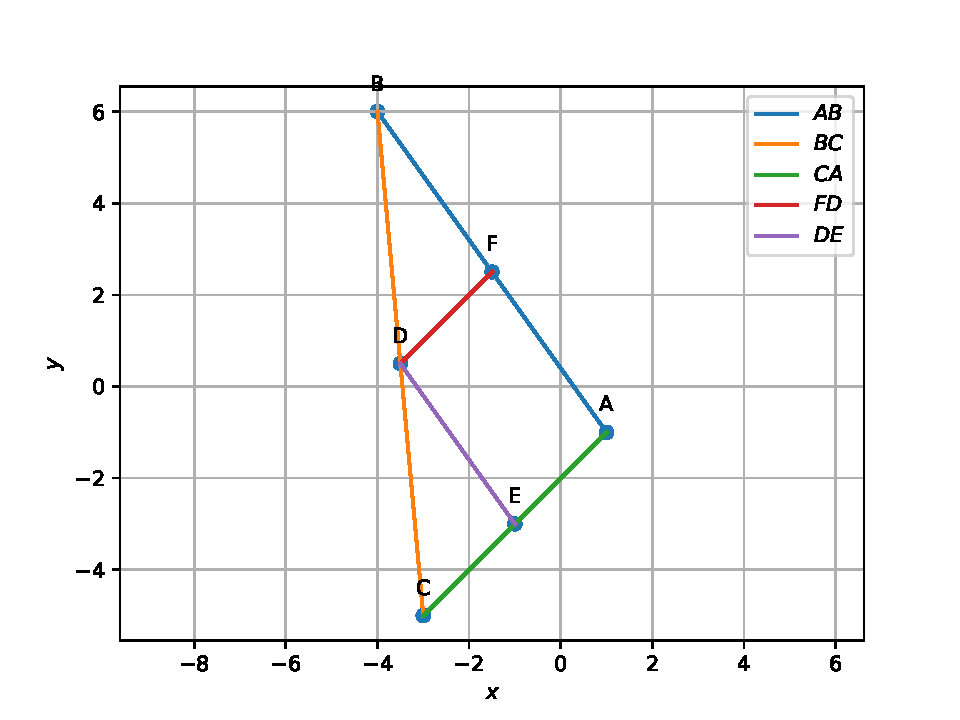
\includegraphics[width=0.75\columnwidth]{figs/triangle/pgm.pdf}
\caption{$AFDE$ forms a parallelogram in triangle ABC}
\label{fig:Triangle-pgm}
\end{figure}






















All codes for this section are available in 
\begin{lstlisting}
	codes/triangle/medians.py
	codes/triangle/pgm.py
\end{lstlisting}
  
\end{enumerate}
